\section{\textsc{Spiegelei}}

\subsection*{Zutaten für 2 Portionen:}

\begin{tabular}{p{7.5cm} p{7.5cm}}
	& \\
	2 Eier & Salz \& Pfeffer \\
	Öl zum Braten & 
\end{tabular}

\subsection*{Serviervorschlag:}

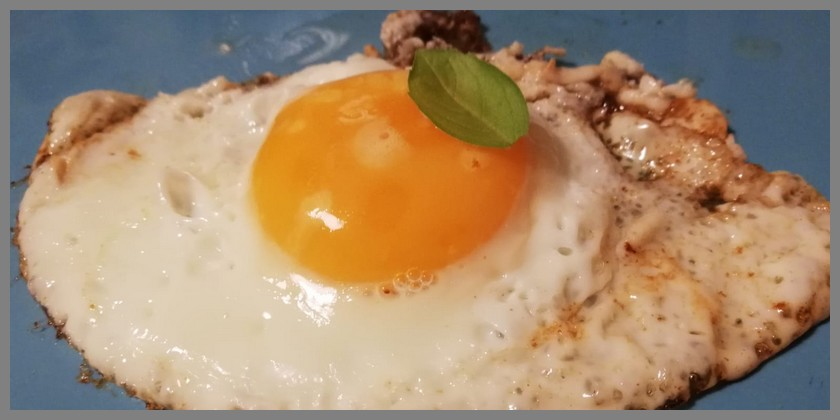
\includegraphics[width=\textwidth]{img/spiegelei.jpg} \cite{spiegelei}

\subsection*{So geht's:}

\begin{tabular}{p{15cm}}
	\\
	Das Öl in einer Pfanne erhitzen.\\
	Ei in das Öl aufschlagen. \\
	Salzen und Deckel auf die Pfanne setzten und je nach Geschmack braten.\\
	Mit einem Pfannenwender das Ei aus der Pfanne nehmen und pfeffern.
\end{tabular}